\documentclass[11pt,a4paper]{article}
\usepackage[T1]{fontenc}
\usepackage[utf8]{inputenc}
\usepackage[magyar]{babel}
\usepackage{lmodern}
\usepackage{amsmath,amssymb}
\usepackage{enumitem}
\usepackage{tikz}
\usetikzlibrary{arrows.meta,patterns}
\usepackage[a4paper,margin=2cm]{geometry}

\pagestyle{empty}
\setlength{\parindent}{0pt}
\setlist[enumerate,1]{label=\textbf{\arabic*.}, leftmargin=*, itemsep=10pt, topsep=3pt}
\setlist[enumerate,2]{label=\alph*), leftmargin=2em, itemsep=4pt, topsep=3pt, parsep=0pt}

\begin{document}

\begin{center}
  {\Large\bfseries Rezgések és mechanikai hullámok -- gyakorló feladatok -- megoldókulcs}
\end{center}

\begin{enumerate}
\item \textbf{Rugós rezgő}
  \begin{enumerate}
    \item $\omega = \sqrt{\dfrac{D}{m}} = \sqrt{\dfrac{80}{0{,}2}} = 20~\tfrac1{\text{s}}$, \quad
      $T = \dfrac{2\pi}{\omega} \approx 0{,}314$~s, \quad $f = \dfrac1T \approx 3{,}18$~Hz.
    \item $v_\text{max} = A\omega = 0{,}04\cdot 20 = 0{,}8~\tfrac{\text{m}}{\text{s}}$, az
      \textbf{egyensúlyi helyzetben};\\
      $a_\text{max} = A\omega^2 = 0{,}04\cdot 400 = 16~\tfrac{\text{m}}{\text{s}^2}$, a
      \textbf{szélső helyzetekben}.
    \item $E = \tfrac12 DA^2 = \tfrac12\cdot 80\cdot 0{,}04^2 = 0{,}064$~J.\\
      $\tfrac12 mv^2 + \tfrac12 Dy^2 = \tfrac12 DA^2 \Rightarrow
      v = \omega\sqrt{A^2 - y^2} = 20\cdot\sqrt{0{,}04^2 - 0{,}02^2} \approx
      0{,}69~\tfrac{\text{m}}{\text{s}}$.
    \item \textbf{(1) Kétszeres tömeg:} $T \propto \sqrt m$, így $T$ $\sqrt2$-szeresére nő
      ($\approx 0{,}44$~s). $\omega$ a $\sqrt2$-ed részére csökken, így
      $v_\text{max} \approx 0{,}57~\tfrac{\text{m}}{\text{s}}$. Az energia
      $\tfrac12 DA^2$ \textbf{nem változik}.\\
      \textbf{(2) Kétszeres amplitúdó:} $T$ \textbf{nem változik}, $v_\text{max}$ kétszeres
      ($1{,}6~\tfrac{\text{m}}{\text{s}}$), az energia négyszeres ($0{,}256$~J).
  \end{enumerate}

\item \textbf{Grafikonelemzés}
  \begin{enumerate}
    \item $A = 3$~cm, $T = 0{,}4$~s, $f = 2{,}5$~Hz, $\omega = 2\pi f \approx 15{,}7~\tfrac1{\text{s}}$.
    \item $v_\text{max} = A\omega \approx 0{,}03\cdot 15{,}7 \approx 0{,}47~\tfrac{\text{m}}{\text{s}}$,
      \quad $a_\text{max} = A\omega^2 \approx 0{,}03\cdot 247 \approx 7{,}4~\tfrac{\text{m}}{\text{s}^2}$.
    \item A sebesség a \textbf{szélső helyzetekben} nulla: $t = 0{,}1$~s és $t = 0{,}3$~s.
      Ugyanekkor a legnagyobb a gyorsulás nagysága, és mindig az egyensúlyi helyzet felé
      mutat: $0{,}1$~s-nál ($y = +3$~cm) lefelé, $0{,}3$~s-nál ($y = -3$~cm) felfelé.
    \item Az ellentétes fázisú rezgés a grafikon tükörképe a $t$ tengelyre
      ($y = -3\sin\omega t$): $0{,}1$~s-nál $-3$~cm, $0{,}3$~s-nál $+3$~cm.\\
      A felső szélső helyzetből induló rezgés kezdőfázisa
      $\varphi_0 = \dfrac{\pi}{2}$ ($90^\circ$): $y = A\sin\left(\omega t + \tfrac{\pi}{2}\right)
      = A\cos\omega t$.
  \end{enumerate}

\item \textbf{Fonálinga és rezonancia}
  \begin{enumerate}
    \item $T = 2\pi\sqrt{\dfrac lg} \Rightarrow l = \dfrac{gT^2}{4\pi^2} =
      \dfrac{9{,}8\cdot 1^2}{39{,}5}~\text{m} \approx 0{,}25$~m.
    \item $T_\text{Hold} = 2\pi\sqrt{\dfrac{0{,}248}{1{,}62}}~\text{s} \approx 2{,}5$~s
      (a $\sqrt{9{,}8/1{,}62} \approx 2{,}46$-szorosa).
    \item $T = \dfrac{44{,}0}{20} = 2{,}2$~s, \quad
      $g = \dfrac{4\pi^2 l}{T^2} = \dfrac{39{,}5\cdot 1{,}2}{2{,}2^2} \approx
      9{,}8~\tfrac{\text{m}}{\text{s}^2}$.\\
      A stopper indításának és leállításának hibája (reakcióidő, kb.\ $0{,}2$~s) egyszer
      jelentkezik. $20$ lengésnél ez $44$~s-hoz képest elhanyagolható, egyetlen $2{,}2$~s-os
      lengésnél viszont kb.\ $10\%$ lenne.
    \item $T = 2\pi\sqrt{\dfrac{2{,}5}{9{,}8}}~\text{s} \approx 3{,}2$~s: kb.\ $3{,}2$
      másodpercenként, mindig ugyanabban a helyzetben (pl.\ a hátsó szélső helyzetből
      indulva). Ez a \textbf{rezonancia}: ha a lökések frekvenciája egyezik a hinta saját
      frekvenciájával, minden lökés a mozgás irányába hat, és növeli az energiát.
    \item A dob forgása periodikus gerjesztést jelent. Felpörgéskor a fordulatszám
      ,,áthalad'' a mosógép (rugókon felfüggesztett üst) saját frekvenciáján: ekkor
      rezonancia lép fel, és nagy a rázkódás. Nagyobb fordulatszámon már messze vagyunk a
      rezonanciától, az amplitúdó újra kicsi (rezonanciagörbe).
  \end{enumerate}

\item \textbf{Hullám a kötélen}
  \begin{enumerate}
    \item $\lambda = 0{,}8$~m, $A = 5$~cm. $c = \lambda f = 0{,}8\cdot 2{,}5 =
      2~\tfrac{\text{m}}{\text{s}}$, \quad $T = \dfrac1f = 0{,}4$~s, \quad
      $t = \dfrac{10~\text{m}}{2~\text{m/s}} = 5$~s.
    \item Kötélhullám: \textbf{transzverzális}; hang a levegőben: \textbf{longitudinális};
      összenyomódás a rugóban: \textbf{longitudinális}; gitárhúr: \textbf{transzverzális}.
      A fény \textbf{nem} mechanikai hullám, hanem elektromágneses: nem kell hozzá közeg,
      vákuumban is terjed.
    \item $\lambda = \dfrac{c}{f} = \dfrac{340}{40\,000}~\text{m} = 8{,}5$~mm.
      A hullám csak a hullámhossznál nagyobb tárgyakról verődik vissza jól; a sokkal kisebb
      tárgyakat a hullám ,,megkerüli'' (elhajlás). A centiméteres rovar a
      $8{,}5$~mm-es ultrahangot visszaveri, a hallható hangot ($\lambda \sim 1$~m) nem.
  \end{enumerate}

\item \textbf{Hullámtörés}
  \begin{enumerate}
    \item $\lambda_1 = \dfrac{c_1}{f} = 0{,}4$~m, \quad $\lambda_2 = \dfrac{c_2}{f} = 0{,}25$~m.
      A \textbf{frekvencia nem változik}: azt a forrás szabja meg, és a határon a két oldal
      pontjai együtt rezegnek.
    \item $\sin\beta = \sin\alpha\cdot\dfrac{c_2}{c_1} = \sin 40^\circ\cdot\dfrac{0{,}5}{0{,}8}
      \approx 0{,}402 \Rightarrow \beta \approx 23{,}7^\circ$.
      A lassabb közegben a hullám a beesési \textbf{merőlegeshez} törik ($\beta < \alpha$).
  \end{enumerate}

\item \textbf{Két hangszóró}
  \begin{enumerate}
    \item $\lambda = \dfrac{340}{680}~\text{m} = 0{,}5$~m.
    \item $\Delta s = 4{,}25 - 3{,}0 = 1{,}25~\text{m} = 2{,}5\lambda = (2\cdot 2+1)\dfrac{\lambda}{2}$:
      \textbf{kioltás}, halk.\\
      $\Delta s = 1{,}0~\text{m} = 2\lambda$: \textbf{erősítés}, hangos.
    \item $\Delta s_\text{min} = \dfrac{\lambda}{2} = 0{,}25$~m.
    \item A falakról, tárgyakról visszaverődő hang további hullámokat ad a hallgató helyén.
      A két hangszóró hangja a különböző távolság miatt nem egyformán erős, így nem
      oltja ki teljesen egymást. A valódi hang sem tisztán egyetlen frekvencia.
  \end{enumerate}

\item \textbf{Gitárhúr}
  \begin{enumerate}
    \item Alaphangnál $L = \dfrac{\lambda}{2}$, tehát $\lambda_1 = 2L = 1{,}2$~m.
      $c = \lambda_1 f_1 = 1{,}2\cdot 330 = 396~\tfrac{\text{m}}{\text{s}}$.
    \item $f_2 = 2f_1 = 660$~Hz, $f_3 = 3f_1 = 990$~Hz.\\[2pt]
      \begin{minipage}[t]{0.5\linewidth}
      Első felhang ($n = 2$): egy teljes hullámhossz fér a húrra. \textbf{3 csomópont} (a két
      végén és középen) és \textbf{2 duzzadóhely} (a negyedeknél).
      \end{minipage}\hfill
      \begin{minipage}[t]{0.45\linewidth}\vspace{0pt}\centering
      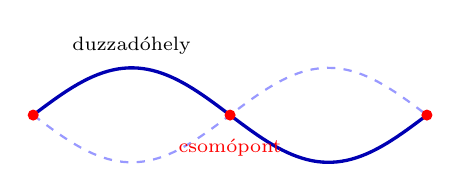
\begin{tikzpicture}[font=\scriptsize]
        \draw[very thick,blue!70!black,domain=0:5,samples=80] plot (\x,{0.6*sin(2*\x/5*180)});
        \draw[thick,blue!40,dashed,domain=0:5,samples=80] plot (\x,{-0.6*sin(2*\x/5*180)});
        \foreach \x in {0,2.5,5} \fill[red] (\x,0) circle (2pt);
        \node[below=5pt,red] at (2.5,0) {csomópont};
        \node[above] at (1.25,0.65) {duzzadóhely};
      \end{tikzpicture}
      \end{minipage}
    \item A hullám sebessége a húron nem változik (ugyanaz a húr, ugyanaz a feszítés):
      $f_1' = \dfrac{c}{2L'} = \dfrac{396}{0{,}9}~\text{Hz} = 440$~Hz (a zenei ,,a'' hang).
  \end{enumerate}

\item \textbf{Szóbeli tétel -- mintaválaszok}

  \textbf{(A) A harmonikus rezgőmozgás.} Rezgőmozgásnak nevezzük azt a mozgást, amelynek
  során a test egy egyensúlyi helyzet körül periodikusan ide-oda mozog. Jellemzői az
  amplitúdó (legnagyobb kitérés), a periódusidő, a frekvencia ($f = 1/T$) és a
  körfrekvencia ($\omega = 2\pi f$). A rezgés harmonikus, ha a kitérés--idő függvény
  szinuszos: $y = A\sin(\omega t + \varphi_0)$, ahol $\omega t + \varphi_0$ a fázis. A
  harmonikus rezgés az egyenletes körmozgás vetülete, ebből
  $v_\text{max} = A\omega$, $a_\text{max} = A\omega^2$, és $a = -\omega^2 y$. Dinamikai
  feltétele a lineáris erőtörvény: az eredő erő arányos a kitéréssel és ellentétes
  irányú, $F = -Dy$. Ebből a rugós rezgő periódusideje $T = 2\pi\sqrt{m/D}$, a kis
  kitérésű fonálingáé $T = 2\pi\sqrt{l/g}$. Egyik sem függ az amplitúdótól. Rezgés közben a
  mozgási és a rugalmas energia egymásba alakul, összegük $E = \tfrac12 DA^2$. A valóságban
  a rezgés csillapodik. Periodikus külső erő hatására kényszerrezgés jön létre, és ha a
  gerjesztés frekvenciája egyezik a saját frekvenciával, az amplitúdó nagyon nagy lesz
  (rezonancia). Példák: hinta, hidak, hangszerek, rádió hangolása.

  \textbf{(B) A mechanikai hullámok.} Ha egy rugalmas közeg egy pontját rezgésbe hozzuk, a
  rezgés továbbterjed a közegben: ez a mechanikai hullám. A hullám energiát és
  rezgésállapotot szállít, anyagot nem, és csak közegben terjed. Transzverzális hullámban a
  részecskék a terjedésre merőlegesen (kötél, húr), longitudinálisban a terjedés irányában
  (hang a levegőben) rezegnek. Jellemzői a hullámhossz, a frekvencia és a terjedési
  sebesség: $c = \lambda f$. A frekvenciát a forrás, a sebességet a közeg határozza meg. A
  közeg határán a hullám visszaverődik (rögzített végen ellentétes fázisban) és megtörik:
  $\sin\alpha/\sin\beta = c_1/c_2$, miközben a frekvencia nem változik. Találkozó hullámok
  kitérései összeadódnak (szuperpozíció). Koherens források esetén interferenciakép jön
  létre: erősítés, ha az útkülönbség $k\lambda$, kioltás, ha $(2k+1)\lambda/2$. A beeső és
  a visszavert hullám interferenciájából állóhullám jön létre, csomópontokkal és
  duzzadóhelyekkel. Két végén rögzített húron $L = n\lambda/2$, ebből adódnak az alaphang és a
  felhangok. A Huygens-elv szerint a hullámfront minden pontja elemi hullámok forrása, ebből
  érthető az elhajlás, amely akkor jelentős, ha a rés mérete a hullámhosszal összemérhető.

  \medskip
  \textbf{Szempontok:} pontos definíciók (amplitúdó, periódusidő, frekvencia,
  hullámhossz); a legfontosabb összefüggések ($a = -\omega^2y$, $T$ képletei, $E$, illetve
  $c = \lambda f$, törési törvény, interferencia-feltételek, $L = n\lambda/2$); legalább egy
  hétköznapi példa minden jelenségre; összefüggő, logikus felépítés.
\end{enumerate}

\end{document}
